\chapter{Sviluppo}
Vengono ora esposte le due "facce" del progetto: il back-end ed il front-end. In particolare ci si soffermerà sul lato client poichè fulcro dell'esperienza finale dell'applicazione.

\section{Architettura Server}
Questo paragrafo ha lo scopo di illustrare la composizione del server che gestisce tutte le funzioni "nascoste" del servizio e il suo funzionamento. A seguire una panoramica generale della sua architettura.

\begin{figure}[!h]
  \centering
    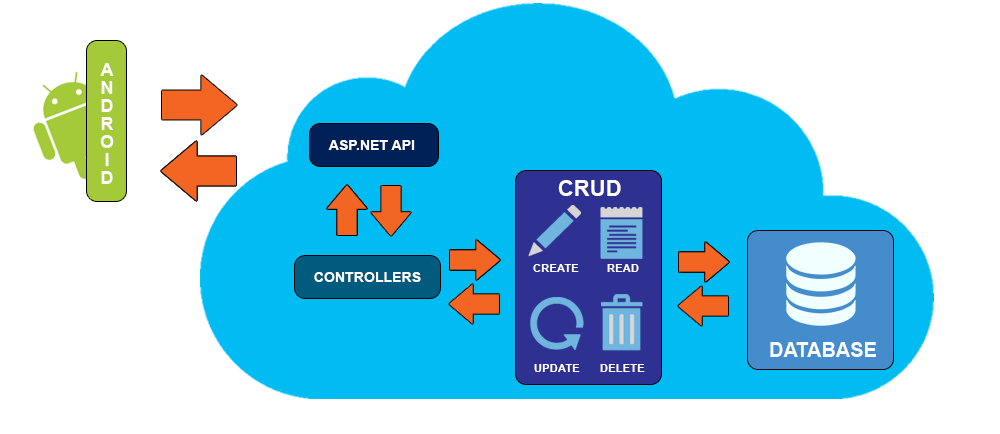
\includegraphics[width=1\textwidth]{server}
  \caption{Architettura server}
  \label{fig:server}
\end{figure}
\FloatBarrier

Il server è basato sulla piattaforma Microsoft Azure, programmato con tecnologia ASP.Net secondo il paradigma MVC (Model-View-Controller). MVC è un pattern architetturale molto diffuso nello sviluppo di sistemi software, in particolare nell'ambito della programmazione orientata agli oggetti, in grado di separare la logica di presentazione dei dati dalla logica di business.
\begin{itemize}
\item \textbf{Model:} rappresentano lo stato dell’applicazione, si occupano della gestione dei dati nel database e contengono i metodi per accedervi. Modifica, lettura e scrittura dei dati sono effettuate secondo il paradigma CRUD. I “risultati” sono inviati tramite View.
\item \textbf{View:} sono responsabili della presentazione dei dati richiesti tramite l’interfaccia utente ed è tramite esse che l’utente invia i comandi ai controllers. Nelle visualizzazioni la quantità di logica è minima e riservata alla presentazione del contenuto. Una view può essere una qualsiasi rappresentazione in output di informazioni, da un semplice grafico alla pagina web di un sito internet.
Come anticipato la View in Android è rappresentata dall'activity.
\item \textbf{Controller:} sono i componenti che gestiscono l’interazione tra l’utente e il Model e selezionano la corretta View da presentare come risultato finale. Nello schema MVC il controller è il punto di partenza poiché seleziona il Model (e relativa View) con cui interagire.
\end{itemize}
È possibile comprendere il funzionamento del paradigma MVC seguendo la semplice creazione di un “percorso” all’interno dell’applicazione.
\begin{enumerate}
\item Tramite l’UI (View) l’utente inizia la creazione del percorso: attraverso la procedura guidata inserisce in un pacchetto JSON tutte le informazioni utili (punto di partenza e arrivo, mezzo utilizzato, prezzo ecc).
\item Completata la procedura di acquisizione informazioni, la View invia i dati al Controller che si occupa della creazione del percorso tramite chiamata https (verso Google).
\item Il controller crea una nuova entità del Model “percorso” con le informazioni inserite dall’utente. Il Model si occuperà dell’inserimento del nuovo percorso nel database.
\item Il Controller aggiorna la View.
\item La View viene aggiornata e l’utente potrà visualizzare il nuovo percorso nell’homepage dell’applicazione.
\end{enumerate}

\section{Contributo personale}
Il mio compito all’interno del team riguardava lo sviluppo dell'interfaccia del progetto destinata all'utente finale. 
Le funzioni a cui mi sono dedicato possono riassumersi nelle seguenti categorie:
\begin{itemize}
\item \textbf{Login e autenticazione:} le operazioni che permettono all’utente di iniziare la propria esperienza d’uso all’interno dell’applicazione, identificandosi con il server e garantendone la sicurezza dei dati forniti tramite il protocollo OAuth. 
\item \textbf{Richieste HTTPS:} la gestione delle richieste verso il server e le risposte da esso con relativi dati allegati. Pertanto è stato necessario studiare e approfondire le meccaniche di funzionamento di una chiamata di REST nell'ecosistema Android.
\item \textbf{User Interface e User Experience:} l’interazione tra client e server tramite comandi grafici e la visualizzazione dei dati ricevuti in risposta (User Interface - UI); il tutto seguendo le linee guida necessarie ad una corretta User eXperience (UX) per mettere a proprio agio l’utente. A tal fine sono state prese in considerazione le risposte degli utenti ai nostri sondaggi.
\end{itemize}
Queste e altre funzioni verranno descritte nel dettaglio nelle sezioni successive.

\section{Architettura Client}
Come detto in precedenza il mio lavoro si è basato principalmente sullo sviluppo del client del nostro servizio ovvero l'applicazione Android con tutti i meccanismi che la compongono.
Di seguito è mostrata una panoramica della sua architettura:

\begin{figure}[!h]
  \centering
    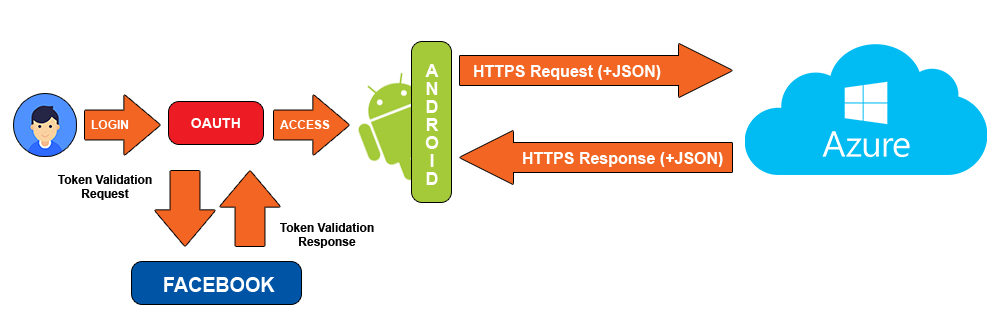
\includegraphics[width=1\textwidth]{client}
  \caption{Architettura client}
  \label{fig:client}
\end{figure}
\FloatBarrier

Il compito del client è di permettere all'utente di compiere operazioni inerenti al servizio a cui è collegato senza che esso sappia come esse vengano eseguite sul server.
L'utente (lo studente in questo caso) si limiterà ad effettuare il login, cercare (o creare) un passaggio e con un "click" potrà prenderne parte.
Vengono ora riportate le funzioni principali sulle quali si è basato il mio lavoro.

\subsection{Autenticazione OAuth}

\begin{wrapfigure}{r}{0.3\textwidth}

\includegraphics[width=0.3\textwidth]{login-button}
\caption{Sezione schermata login}
\label{fig:login-button}
\end{wrapfigure} 
\FloatBarrier

La prima schermata che l'utente incontrerà sarà quella di login.
È stato necessario trovare un metodo di login sicuro, che rientrasse nei parametri “user-friendly” ovvero gradevole alla vista e di facile utilizzo e che permettesse di identificare automaticamente molte informazioni dell’utente per velocizzare la procedura di registrazione. Tra le molteplici soluzioni possibili si è optato per l’accesso con protocollo OAuth tramite API Facebook.
OAuth è un protocollo aperto che permette ad un service provider (in questo caso Facebook) di condividere le informazioni personali di un utente con un consumer (in questo caso MoveMate) senza cedere le credenziali personali, il tutto ovviamente con il consenso dell'utente. È stato scelto questo metodo per poter unire la diffusione e facilità di utilizzo del servizio Facebook e la sicurezza del protocollo OAuth.
Alla pressione del pulsante di login (Figura \ref{fig:login-button}) inizierà il processo di autenticazione. Il tutto è gestito da una chiamata asincrona verso il server Facebook contenente un token di identificazione che verrà confermato lato server. Come mostrato nel listato \ref{lst:callback} la chiamata gestisce tre casi:

\begin{itemize}
\item \textbf{onSuccess:} rappresenta il caso di successo dell'autenticazione. Verrà chiamata la funzione interna check() detta callback\footnote{In programmazione, una callback è, in genere, una funzione, o un "blocco di codice" che viene passata come parametro ad un'altra funzione.} per il controllo dei dati utenti, in grado di verificare se si tratta di un utente già registrato o meno.
\item \textbf{onCancel:} è il caso in cui l'utente cancella la procedura di autenticazione prima del suo completamento. Nel nostro caso non verrà eseguita nessuna funzione e l'utente rimarrà nella schermata di login.
\item \textbf{onError:} indica il caso in cui sopraggiunga un errore di qualunque tipo e verrà mostrato il messaggio di errore a schermo.
\end{itemize}

In seguito al primo login (quindi nella funzione check()) è stato inserito un wizard\footnote{Nel linguaggio dell'informatica, il wizard (o autocomposizione) indica una procedura informatica, generalmente inglobata in una applicazione più complessa, che permette all'utente di eseguire determinate operazioni (solitamente complesse) tramite una serie di passi successivi.} che guida l’utente nella procedura di associazione tra il proprio profilo Facebook, le proprie credenziali universitarie (ateneo, matricola, email) e numero di telefono necessario per essere contattato dagli altri utenti.
Per la verifica dello status di studente e quindi garantire la partecipazione alla nostra community ai soli studenti, è stato implementato un sistema di verifica della casella di posta elettronica universitaria tramite invio e verifica di un codice univoco. Una volta terminata la procedura di identificazione iniziale, l’utente sarà in grado di accedere all’applicazione in maniera automatica grazie alle API Facebook e all’associazione ID Facebook – Email Studente.
Da questo momento in poi l'applicazione (precisamente il server) avrà tutti i dati dell'utente necessari al funzionamento del servizio.

\bigskip
\begin{minipage}{\linewidth}
\begin{lstlisting}[language=Java, caption=Esempio Facebook callback, label={lst:callback}]
FacebookSdk.sdkInitialize(getApplicationContext());
callbackManager = CallbackManager.Factory.create();
loginButton = (LoginButton) findViewById(R.id.login_button);
loginButton.registerCallback(callbackManager, new FacebookCallback<LoginResult>() {
            @Override
            public void onSuccess(LoginResult loginResult) {
                check();
            }

            @Override
            public void onCancel() {

            }

            @Override
            public void onError(FacebookException exception) {
                Toast.makeText(LoginActivity.this, "Errore: " + exception,Toast.LENGTH_LONG).show();
            }
        });
\end{lstlisting}
\end{minipage}
\FloatBarrier

\subsection{Richieste HTTPS}
Bisogna ricordare che la maggior parte dei calcoli necessari al funzionamento dell'applicazione sono eseguiti sul server che restituisce dei risultati visibili dall'utente. La singola pressione di un pulsante può attivare una semplice funzione con l'unico scopo di inviare un comando al back-end che "ritornerà" il risultato richiesto.
L’invio di comandi al server è reso possibile tramite chiamate REST: richieste e risposte sono inviate tramite protocollo HTTP all’interno di una connessione criptata con protocollo SSL per garantire l’autenticità del sito web, la protezione della privacy degli utenti e l’integrità dei dati scambiati tra applicazione e database. Android mette a disposizione la propria libreria “Volley” che permette di gestire richieste, risposte ed eventuali errori rendendo leggibile e compatto il codice. Il listato \ref{lst:https} mostra un esempio di chiamata REST nell’ecosistema Android che come nel processo di login si divide in due casi: la funzione onResponse() gestisce le operazioni da eseguire quando lo status code della risposta è 200, ovvero nel caso in cui la chiamata al server abbia avuto esito positivo, mentre la funzione onErrorResponse() si occupa di gestire le varie eccezioni in caso di errori (status code 400, 404 ecc.). 
Le richieste vengono gestite da controllers all’interno del server che rispondono con le informazioni richieste solo previa autenticazione dell'utente. Richieste e risposte sono spesso accompagnate da pacchetti di tipo JSON, ovvero informazioni di tipo attributo-valore codificato in modo tale da essere di facile comprensione, per inviare i parametri alle funzioni del server o i risultati richiesti dall’applicazione.
\bigskip
\begin{minipage}{\linewidth}
\begin{lstlisting}[language=java, caption=Esempio richiesta https,label={lst:https}]
RequestQueue queue = Volley.newRequestQueue(ctx);
String url = // url funzione server
StringRequest stringRequest = new StringRequest( /* request */ type, url,
    new Response.Listener<String>() {
        @Override
        public void onResponse(String response) {
			// successo                                               
            }
    },
    new Response.ErrorListener() {
        @Override
        public void onErrorResponse(VolleyError error) {
        	// gestione errore
        }
    }
);
queue.add(stringRequest); 
\end{lstlisting}
\end{minipage}
\FloatBarrier

\subsection{Interfaccia User-Friendly}
Poiché “anche l’occhio vuole la sua parte”, una sezione fondamentale del progetto è stata la realizzazione di un’interfaccia grafica di qualità e che mettesse l’utente a proprio agio già dal primo utilizzo. L'esperienza utente è ciò che una persona prova quando utilizza un prodotto o un servizio ed è fondamentale cercare di renderla il più gradevole possibile affinchè l'utente finale possa trovarne giovamento e venga fidelizzato: ciò garantirà il suo utilizzo anche in futuro.
Sono stati effettuati numerosi mockup, successivamente sottoposti all’utente per verificarne l’usabilità. La grafica è ispirata ai vari competitor di successo con l'adattamento al target del nostro progetto, ovvero gli studenti, mettendo in risalto informazioni specifiche per loro come i dipartimenti a cui afferiscono.
I feedback riportati dagli utenti che hanno provato il prototipo dell’applicazione sono stati ascoltati e applicati per arrivare alla versione finale. Di seguito due esempi delle modifiche applicate durante il progetto.

\begin{figure}[!h]
  \centering
\begin{minipage}[c]{\linewidth}
  \centering
    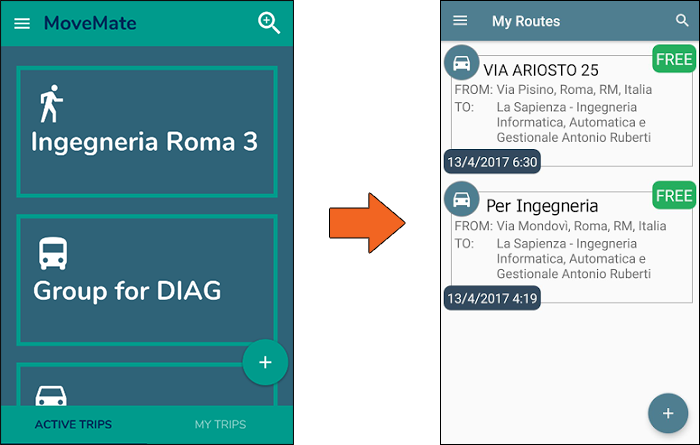
\includegraphics[width=1\textwidth]{path}
  \caption{Lista percorsi disponibili (prima e dopo)}
  \label{fig:path}
\bigskip
  \centering
    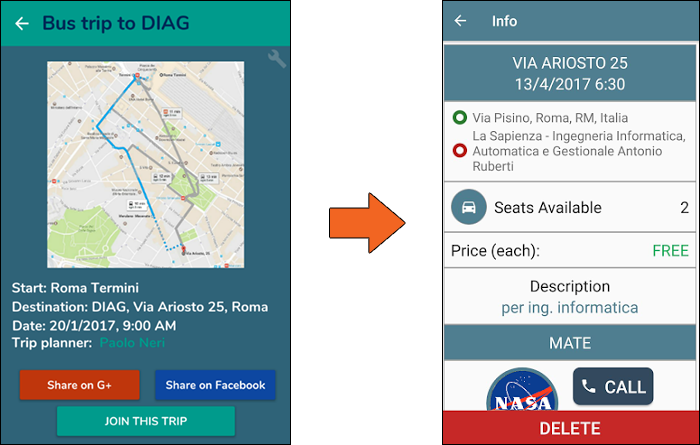
\includegraphics[width=1\textwidth]{path-info}
  \caption{Dettagli percorso (prima e dopo)}
  \label{fig:path-info}
\end{minipage}
\end{figure}
\FloatBarrier


\subsection{Librerie esterne}
Il lavoro necessario a completare tutte le funzioni dell'applicazione sarebbe diventato estenuante senza l'uso delle librerie, native e non.
Per implementare features preesistenti e per poter rendere il codice modulare e intuitivo sono state usate librerie provenienti prevalentemente dalla piattaforma GitHub\footnote{GitHub è un servizio di hosting per progetti software prevalentemente open-source. Il nome "GitHub" deriva dal fatto che GitHub è una implementazione dello strumento di controllo versione distribuito Git.}, piattaforma per la condivisione di progetti software, oltre a quelle proprietarie di Google. A tal fine, GitHub ha dato modo di esplorare sul campo il concetto di opensource che ha permesso di velocizzare e semplificare il lavoro, senza dover scrivere da zero porzioni di codice già esistenti. L’ecosistema Android, ben predisposto all’utilizzo di librerie esterne, ha garantito infine una rapida assimilazione del concetto di libreria fino a quel momento a me sconosciuto dal punto di vista pratico.
Le librerie usate spaziano dall’arricchimento della grafica per un migliore feedback da parte dell’utente, al download e compressione delle immagini per rendere l’applicazione e il carico verso il server leggeri, fino alla creazione dei percorsi sui quali si basa l'applicazione. Punto focale della descrizione di ogni percorso, infatti, è la mappa dello stesso.
Per integrarla nel progetto è stata usata la libreria Android-GoogleDirectionLibrary\footnote{\url{https://github.com/akexorcist/Android-GoogleDirectionLibrary}} che si occupa di creare il percorso, con il mezzo selezionato dall’utente, tramite chiamate REST verso i server Google.
Dati un punto di partenza e uno di arrivo, viene generato (onDirectionSuccess) un tracciato automatico sulla mappa che consente ai potenziali passeggeri di visualizzare l’ipotetico percorso che si effettuerà durante il viaggio.
La libreria sfrutta le API Google Maps che necessitano di una serverKey, generata nella Google API Console, per autenticare sviluppatore e applicazione e garantirne la proprietà.
\bigskip
\begin{minipage}{\linewidth}
\begin{lstlisting}[language=java, caption=Esempio integrazione Google API]
String serverKey = "AIzaSyDFWdlR5DG1VYXSaMwG62ilxxxxxxxxx";
LatLng origin = new LatLng(37.7849569, -122.4068855);
LatLng destination = new LatLng(37.7814432, -122.4460177);
String transitMode = TransportMode.DRIVING;
GoogleDirection.withServerKey(serverKey)
    .from(origin)
    .to(destination)
    .transitMode(transitMode)
    .execute(new DirectionCallback() {
        @Override
        public void onDirectionSuccess(Direction direction, String rawBody) {
            // successo 
        }

        @Override
        public void onDirectionFailure(Throwable t) {
            // gestione errore 
        }
    });
\end{lstlisting}
\end{minipage}
\FloatBarrier

